%% 
%% Copyright 2007, 2008, 2009 Elsevier Ltd
%% 
%% This file is part of the 'Elsarticle Bundle'.
%% ---------------------------------------------
%% 
%% It may be distributed under the conditions of the LaTeX Project Public
%% License, either version 1.2 of this license or (at your option) any
%% later version.  The latest version of this license is in
%%    http://www.latex-project.org/lppl.txt
%% and version 1.2 or later is part of all distributions of LaTeX
%% version 1999/12/01 or later.
%% 
%% The list of all files belonging to the 'Elsarticle Bundle' is
%% given in the file `manifest.txt'.
%% 

%% Template article for Elsevier's document class `elsarticle'
%% with numbered style bibliographic references
%% SP 2008/03/01

\documentclass[preprint,12pt,a4paper]{elsarticle}



%% Use the option review to obtain double line spacing
%% \documentclass[authoryear,preprint,review,12pt]{elsarticle}

%% For including figures, graphicx.sty has been loaded in
%% elsarticle.cls. If you prefer to use the old commands
%% please give \usepackage{epsfig}

%% The amssymb package provides various useful mathematical symbols
%% \usepackage{amssymb}
\usepackage{hyperref}
\setlength{\parindent}{0pt}
%% The amsthm package provides extended theorem environments
%% \usepackage{amsthm}

%% The lineno packages adds line numbers. Start line numbering with
%% \begin{linenumbers}, end it with \end{linenumbers}. Or switch it on
%% for the whole article with \linenumbers.
% \usepackage{lineno}
\usepackage{tabularray}
\usepackage{float}
\usepackage[T1]{fontenc}
% \usepackage{helvet}
\renewcommand{\familydefault}{\sfdefault}
\newcommand{\tab}[1]{\hspace{.2\textwidth}\rlap{#1}}

\journal{SoftwareX}

\begin{document}


    \renewcommand{\labelenumii}{\arabic{enumi}.\arabic{enumii}}

    \begin{frontmatter}

        \title{\textbf{quicR}:\ An R Library for Streamlined Data Handling of Real-Time Quaking Induced Conversion Assays}
        \author[label1,label2,label3]{Gage Rowden\corref{cor}}
        \fntext[ ]{\textit{E-mail address: }rowde002@umn.edu}
        \cortext[cor]{Corresponding author.}
        \author[label1,label2,label3]{Peter Larsen}
        \address[label1]{Department of Veterinary and Biomedical Sciences, University of Minnesota, USA.}
        \address[label2]{Minnesota Center for Prion Research and Outreach, University of Minnesota, USA.}
        \address[label3]{Priogen Corp., USA.}

        \begin{abstract}
            Real-time quaking induced conversion (RT-QuIC) has become a valuable diagnostic tool for protein misfolding disorders such as Creutzfeldt-Jakob disease and Parkinson's disease. Given that the technology is relatively new, academic and industry standards for quality filtering data and high throughput analysis of results have yet to be fully established. The open source R library, \textbf{quicR}, was developed to provide a standardized approach to RT-QuIC data analysis.\ \textbf{quicR} provides functions, which can be easily integrated into existing R workflows, for data curation, analysis, and visualization.
        \end{abstract}

        \begin{keyword}
            R package \sep{} RT-QuIC \sep{} prion \sep{} diagnostics \sep{} CJD \sep{} Parkinson's
        \end{keyword}

    \end{frontmatter}

    % \linenumbers

    \section*{Metadata}

    \begin{table}[ht]
        \fontsize{9pt}{9pt}\selectfont
        \centering
        \begin{tabular}{lp{6cm}p{6cm}}
            \hline{}
            \textbf{Nr.} & \textbf{Code metadata description} & \textbf{Metadata} \\
            \hline{}
            C1 & Current code version & V2.1.0 \\
            % \hline{}
            C2 & Permanent link to code/repository used for this code version & \url{https://github.com/gage1145/quicR/releases/tag/v2.1.0} \\
            % \hline{}
            C3  & Permanent link to Reproducible Capsule & \url{https://cran.r-project.org/web/packages/quicR}\\
            % \hline{}
            C4 & Legal Code License & GPL-3 \\
            % \hline{}
            C5 & Code versioning system used & Git \\
            % \hline{}
            C6 & Software code languages, tools, and services used & R \\
            % \hline{}
            C7 & Compilation requirements, operating environments \& dependencies & R (>=4.1.0) \\
            % \hline{}
            C8 & If available Link to developer documentation/manual & \url{https://cran.r-project.org/web/packages/quicR/quicR.pdf}\\
            % \hline{}
            C9 & Support email for questions & rowde002@umn.edu\\
            \hline{}
        \end{tabular}
    \end{table}

    \section{Motivation and significance}
        Real-time quaking induced conversion (RT-QuIC) is a cutting-edge diagnostic assay that has garnered significant attention for its ultra-sensitive detection of misfolded protein aggregates \cite{Wilham2010, Atarashi2011}. The assay works by converting a recombinant protein substrate into an amyloid aggregate in the presence of a misfolded seed \cite{Wilham2010, Orru2012, Orru2017, Orru2015, Bongianni2019, Dassanayake2016, Hwang2018, Groveman2018, Metrick2020}. The assay's sensitivity and specificity make RT-QuIC a promising tool for diagnosing diseases such as prion disorders and other protein misfolding pathologies \cite{Fiorini2020, Franceschini2017, Picasso-Risso2022, Holz2021}. However, the relatively recent development and novelty of the assay have left a gap in widely accepted academic and industry standards for data analysis and interpretation \cite{Rowden2023}.

        To address this gap, we introduce \textbf{quicR}, an open-source library, developed in R \cite{R2024}, dedicated to the cleaning, analysis, and visualization of RT-QuIC data. By consolidating key metrics and providing robust analytical tools, \textbf{quicR} aims to standardize the analysis pipeline and foster reproducibility within the field of quaking induced assays including related assays such as Nano-QuIC \cite{Christenson2023} and Micro-QuIC \cite{Lee2024}. \textbf{quicR} is designed with both researchers and diagnosticians in mind, providing a user-friendly interface that integrates seamlessly with existing R workflows.

        While universal diagnostic criteria for RT-QuIC have yet to be established, certain analytical metrics have emerged as valuable tools for interpreting assay results and kinetics. These include:

        \begin{enumerate}
            \item Time-to-threshold (TtT): The time required for the fluorescence signal to exceed a predefined threshold \cite{Orru2015}.
            \item Rate of amyloid formation (RAF): A measure of the kinetics of aggregate growth, which provides insight into the relative quantity of misfolded seed \cite{Gallups2022}.
            \item Maxpoint ratio (MPR): A ratio-based metric measuring peak normalized fluorescence intensities \cite{Rowden2023}.
            \item Maximum slope (MS): The steepest rate of fluorescence increase, reflecting the most rapid phase of aggregation \cite{Henderson2015}.
        \end{enumerate}

        Together, these metrics enable researchers to characterize the kinetics of RT-QuIC reactions comprehensively, enhancing the rigor and reliability of diagnostic decisions.

        In addition to analytical tools, \textbf{quicR} provides flexible and customizable visualization capabilities. Leveraging the powerful ggplot2 library \cite{ggplot2016}, \textbf{quicR} enables users to generate high-quality, publication-ready figures. These visualizations can be further customized using the intuitive `+' syntax of ggplot2, allowing for tailored presentations of RT-QuIC data.

        By combining standardized metrics, advanced visualization tools, and a commitment to open source science, \textbf{quicR} serves as a foundational tool to empower researchers to analyze and present RT-QuIC data with clarity, consistency, and cohesion.

    \section{Software description}
        \subsection{Software architecture}
            \textbf{quicR} was developed to address the growing need for efficient data conversion, analysis, and visualization of RT-QuIC data (Figure \ref{fig:workflow}). With a focus on usability and reproducibility, the package is designed to standardize workflows and ensure compatibility across multiple laboratories. The overall architecture revolves around integration with the proprietary MARS software (BMG Labtech, Ortenberg, Germany) which exports raw data as Excel workbooks. The data from these workbooks is then curated into usable objects in the R environment, and visualized.

            \begin{figure}[ht]
                \centering
                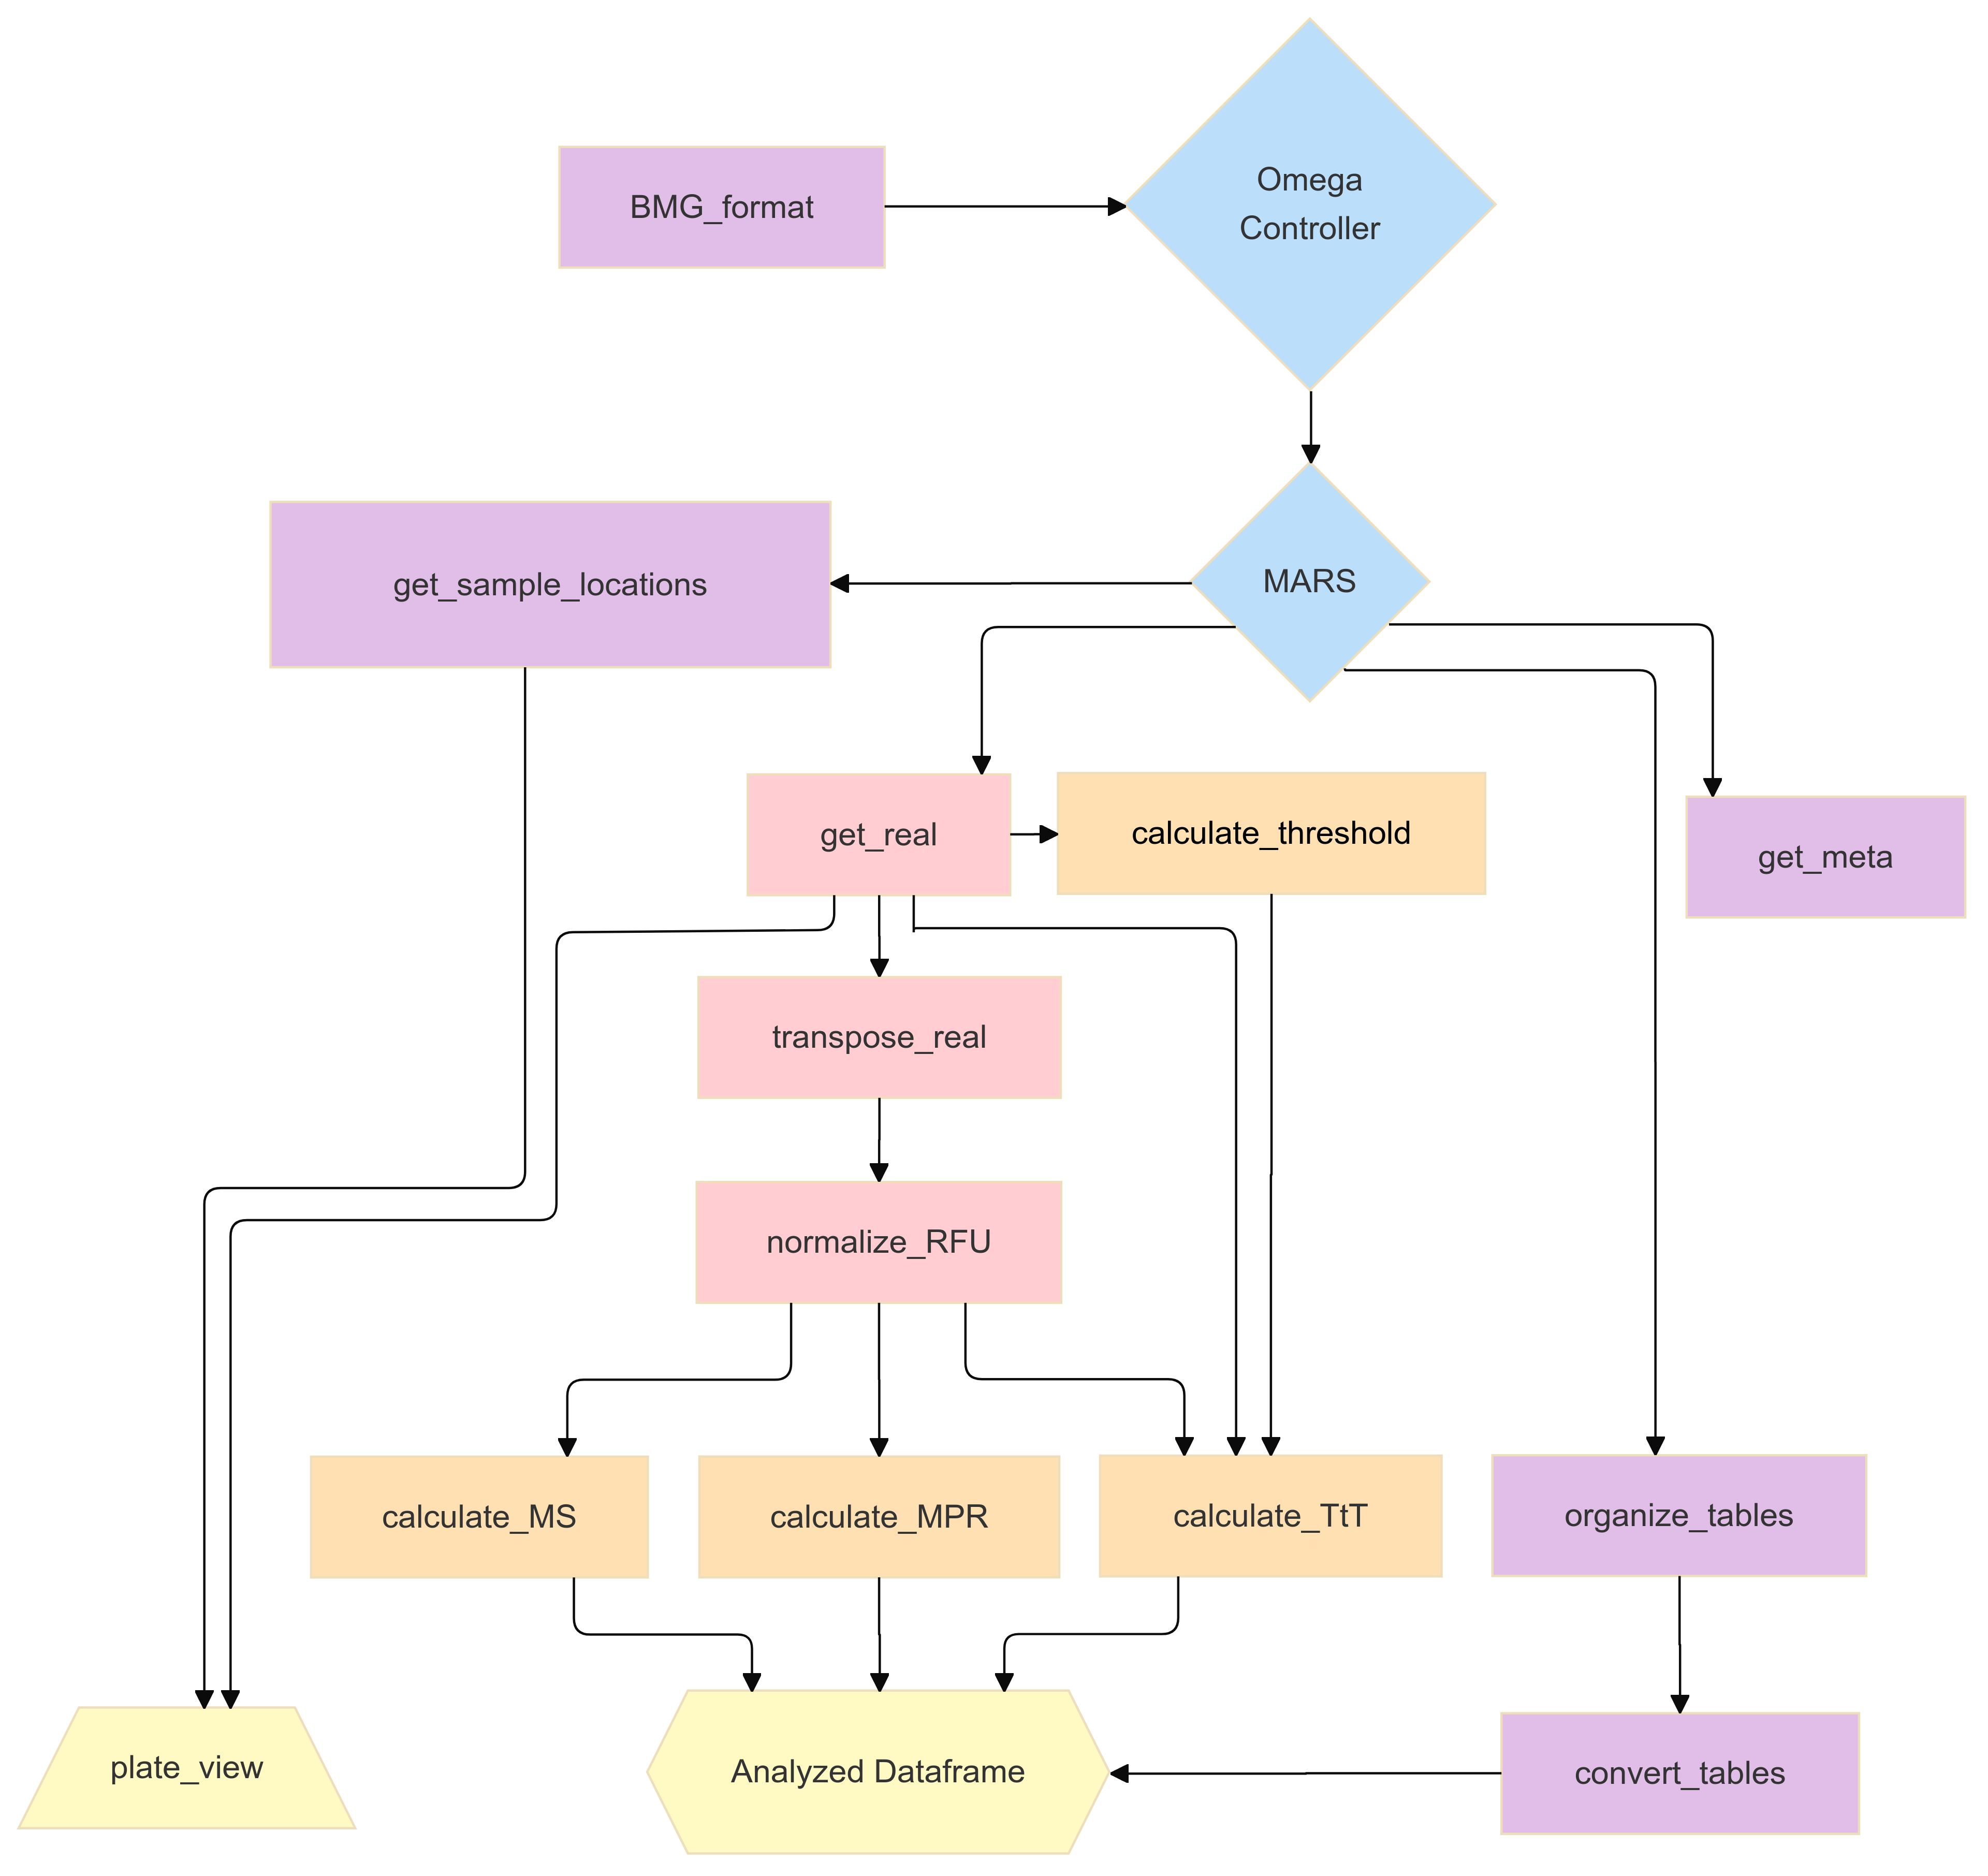
\includegraphics[width=\textwidth]{images/workflow.png}
                \caption{Workflow hierarchy of the \textbf{quicR} package. Blue nodes indicate steps where BMG software is needed. Purple nodes indicate functions dedicated to handling metadata. Red nodes are functions that acquire and manipulate raw data. Orange nodes are functions which calculate some metric. Finally, yellow nodes represent data analysis endpoints.}
                \label{fig:workflow}
            \end{figure}

    \subsection{Software functionalities}
        The implementation of the \textbf{quicR} package encompasses several streamlined processes designed to facilitate data input, cleaning, transformation, and analysis of RT-QuIC data. This section provides a comprehensive guide to utilizing the package's key functionalities, detailing how to:
            
        \begin{enumerate}
            \item Format and input sample data into Omega control software (BMG Labtech, Ortenberg, Germany).
            \item Extract, clean, and organize metadata and raw data and apply transformations/normalization for downstream analysis.
            \item Calculate critical analytical metrics, such as time-to-threshold (TtT), rate of amyloid formation (RAF), maxpoint ratio (MPR), and maximum slope (MS).
            \item Visualize raw and analyzed data.
        \end{enumerate}

        These steps are designed to enhance reproducibility, minimize manual data handling, and enable seamless integration with the MARS software workflow.

        \subsubsection{Input of Sample IDs into Omega Control Software}
            The Omega control software allows input of a TXT file containing sample IDs, dilution factors, and their well locations. This file is uniquely formatted, and not easily reproduced manually.

            \begin{enumerate}
                \item \textbf{BMG\_format()}: This function allows for input of a CSV file containing the plate layout (see Table \ref{tbl:layout} for proper formatting), and exports the formatted TXT file. The file can then be imported into the Omega control software before running.
            \end{enumerate}
            
            \begin{table}[ht]
                \centering
                \begin{tblr}{
                    cells     = {font = \fontsize{11pt}{11pt}\selectfont},
                    colspec   = {|c|cccccccccccc|}, 
                    row{1}    = {font=\bfseries}, 
                    column{1} = {font=\bfseries}, 
                    rowhead   = 1,
                    width     = \textwidth
                }
                    \hline
                    & 1 & 2 & 3 & 4 & 5 & 6 & 7 & 8 & 9 & 10 & 11 & 12 \\ 
                    \hline
                    A & P & S01 & S02 & S03 & S04 & S05 & S06 & S07 & S08 & S09 & S10 & S11 \\ 
                    B & P & S01 & S02 & S03 & S04 & S05 & S06 & S07 & S08 & S09 & S10 & S11 \\ 
                    C & P & S01 & S02 & S03 & S04 & S05 & S06 & S07 & S08 & S09 & S10 & S11 \\ 
                    D & P & S01 & S02 & S03 & S04 & S05 & S06 & S07 & S08 & S09 & S10 & S11 \\ 
                    E & N & S01 & S02 & S03 & S04 & S05 & S06 & S07 & S08 & S09 & S10 & S11 \\ 
                    F & N & S01 & S02 & S03 & S04 & S05 & S06 & S07 & S08 & S09 & S10 & S11 \\ 
                    G & N & S01 & S02 & S03 & S04 & S05 & S06 & S07 & S08 & S09 & S10 & S11 \\ 
                    H & N & S01 & S02 & S03 & S04 & S05 & S06 & S07 & S08 & S09 & S10 & S11 \\ 
                    \hline
                \end{tblr}
                \caption{Example CSV file plate layout for input into the ``BMG\_format'' function. The top left corner should be cell ``A1'' in the CSV file. The top numbered row and the left-most lettered column should never be altered.}
                \label{tbl:layout}
            \end{table}

        \subsubsection{Data Cleaning and Transformation}
            The MARS software exports real-time data as an Excel workbook. Typically, the first sheet in the workbook will include microplate views of both raw data and metadata; however, the metadata on this page is what is most useful for downstream processes. Those tables include the ``Sample IDs'' and ``Dilutions'' tables (if dilutions were included in the MARS export). For much of the downstream analysis, it is crucial that the ``Sample IDs'' table was exported from MARS.\@ If there is no table, the user can simply add it manually.

            \begin{enumerate}
                \item \textbf{organize\_tables()}: returns a list of tables contained in the first sheet of the exported Excel sheet. These tables contain valuable metadata such as sample IDs, dilution factors, and microplate locations.
                \item \textbf{convert\_tables()}: accepts tables outputted from \textbf{organize\_tables} and converts them to columns in a data frame.
                \item \textbf{get\_sample\_locations()}: extracts the well locations for each sample. Output of this function is used as an argument for visualizing a microplate-level view of real-time data.
            \end{enumerate}

        \subsubsection{Retrieving and Manipulating Raw Data}
            The raw, real-time data is typically found on the second sheet of the Excel workbook exported from MARS. There are three functions dedicated to the retrieval and cleaning of raw data.

            \begin{enumerate}
                \item \textbf{get\_real()}: Retrieves the raw data from the Excel file, and outputs it as a data frame.
                \item \textbf{transpose\_real()}: Swaps the rows and columns which makes some downstream analyses easier.
                \item \textbf{normalize\_RFU()}: normalizes the raw data by dividing each read by background fluorescence at a given cycle.
            \end{enumerate}

        \subsubsection{Calculations}
            Three analytical metrics have dedicated functions: time-to-threshold (TtT), maxpoint ratio (MPR), and maximum slope (MS). The rate of amyloid formation (RAF) does not have a designated function since it is simply the reciprocal of the time-to-threshold (1/TtT). However, it can be calculated using the calculate\_metrics() function if TtT is chosen as an optional parameter. Each function below accepts input from the transpose\_real() or the normalize\_RFU() functions. See Figure \ref{fig:metrics} for an example of the output of these functions.

            \begin{enumerate}
                \item \textbf{calculate\_threhold()}: returns a value which is a given number of standard deviations above the average background fluorescence of the entire microplate. This is a popular method of threshold calculation as reviewed in Rowden, et al.\cite{Rowden2023}.
                \item \textbf{calculate\_TtT()}: takes the real-time data and calculates the time in hours needed to reach a given threshold value. This threshold can be supplied by calculate\_threshold() or determined separately by the user.
                \item \textbf{calculate\_MPR()}: accepts raw or normalized data and returns the maximum value obtained during the run. If supplied with raw data, it will make a call to the normalize\_RFU() function.
                \item \textbf{calculate\_MS()}: computes the approximate derivative of the real-time data and returns the maximum value obtained during the run.
                \item \textbf{calculate\_metrics()}: makes a call to functions 2--4 above and generates a data frame with the sample-matched metrics. Also computes RAF if TtT is given as an argument.
            \end{enumerate}

            \begin{figure}[ht]
                \centering{}
                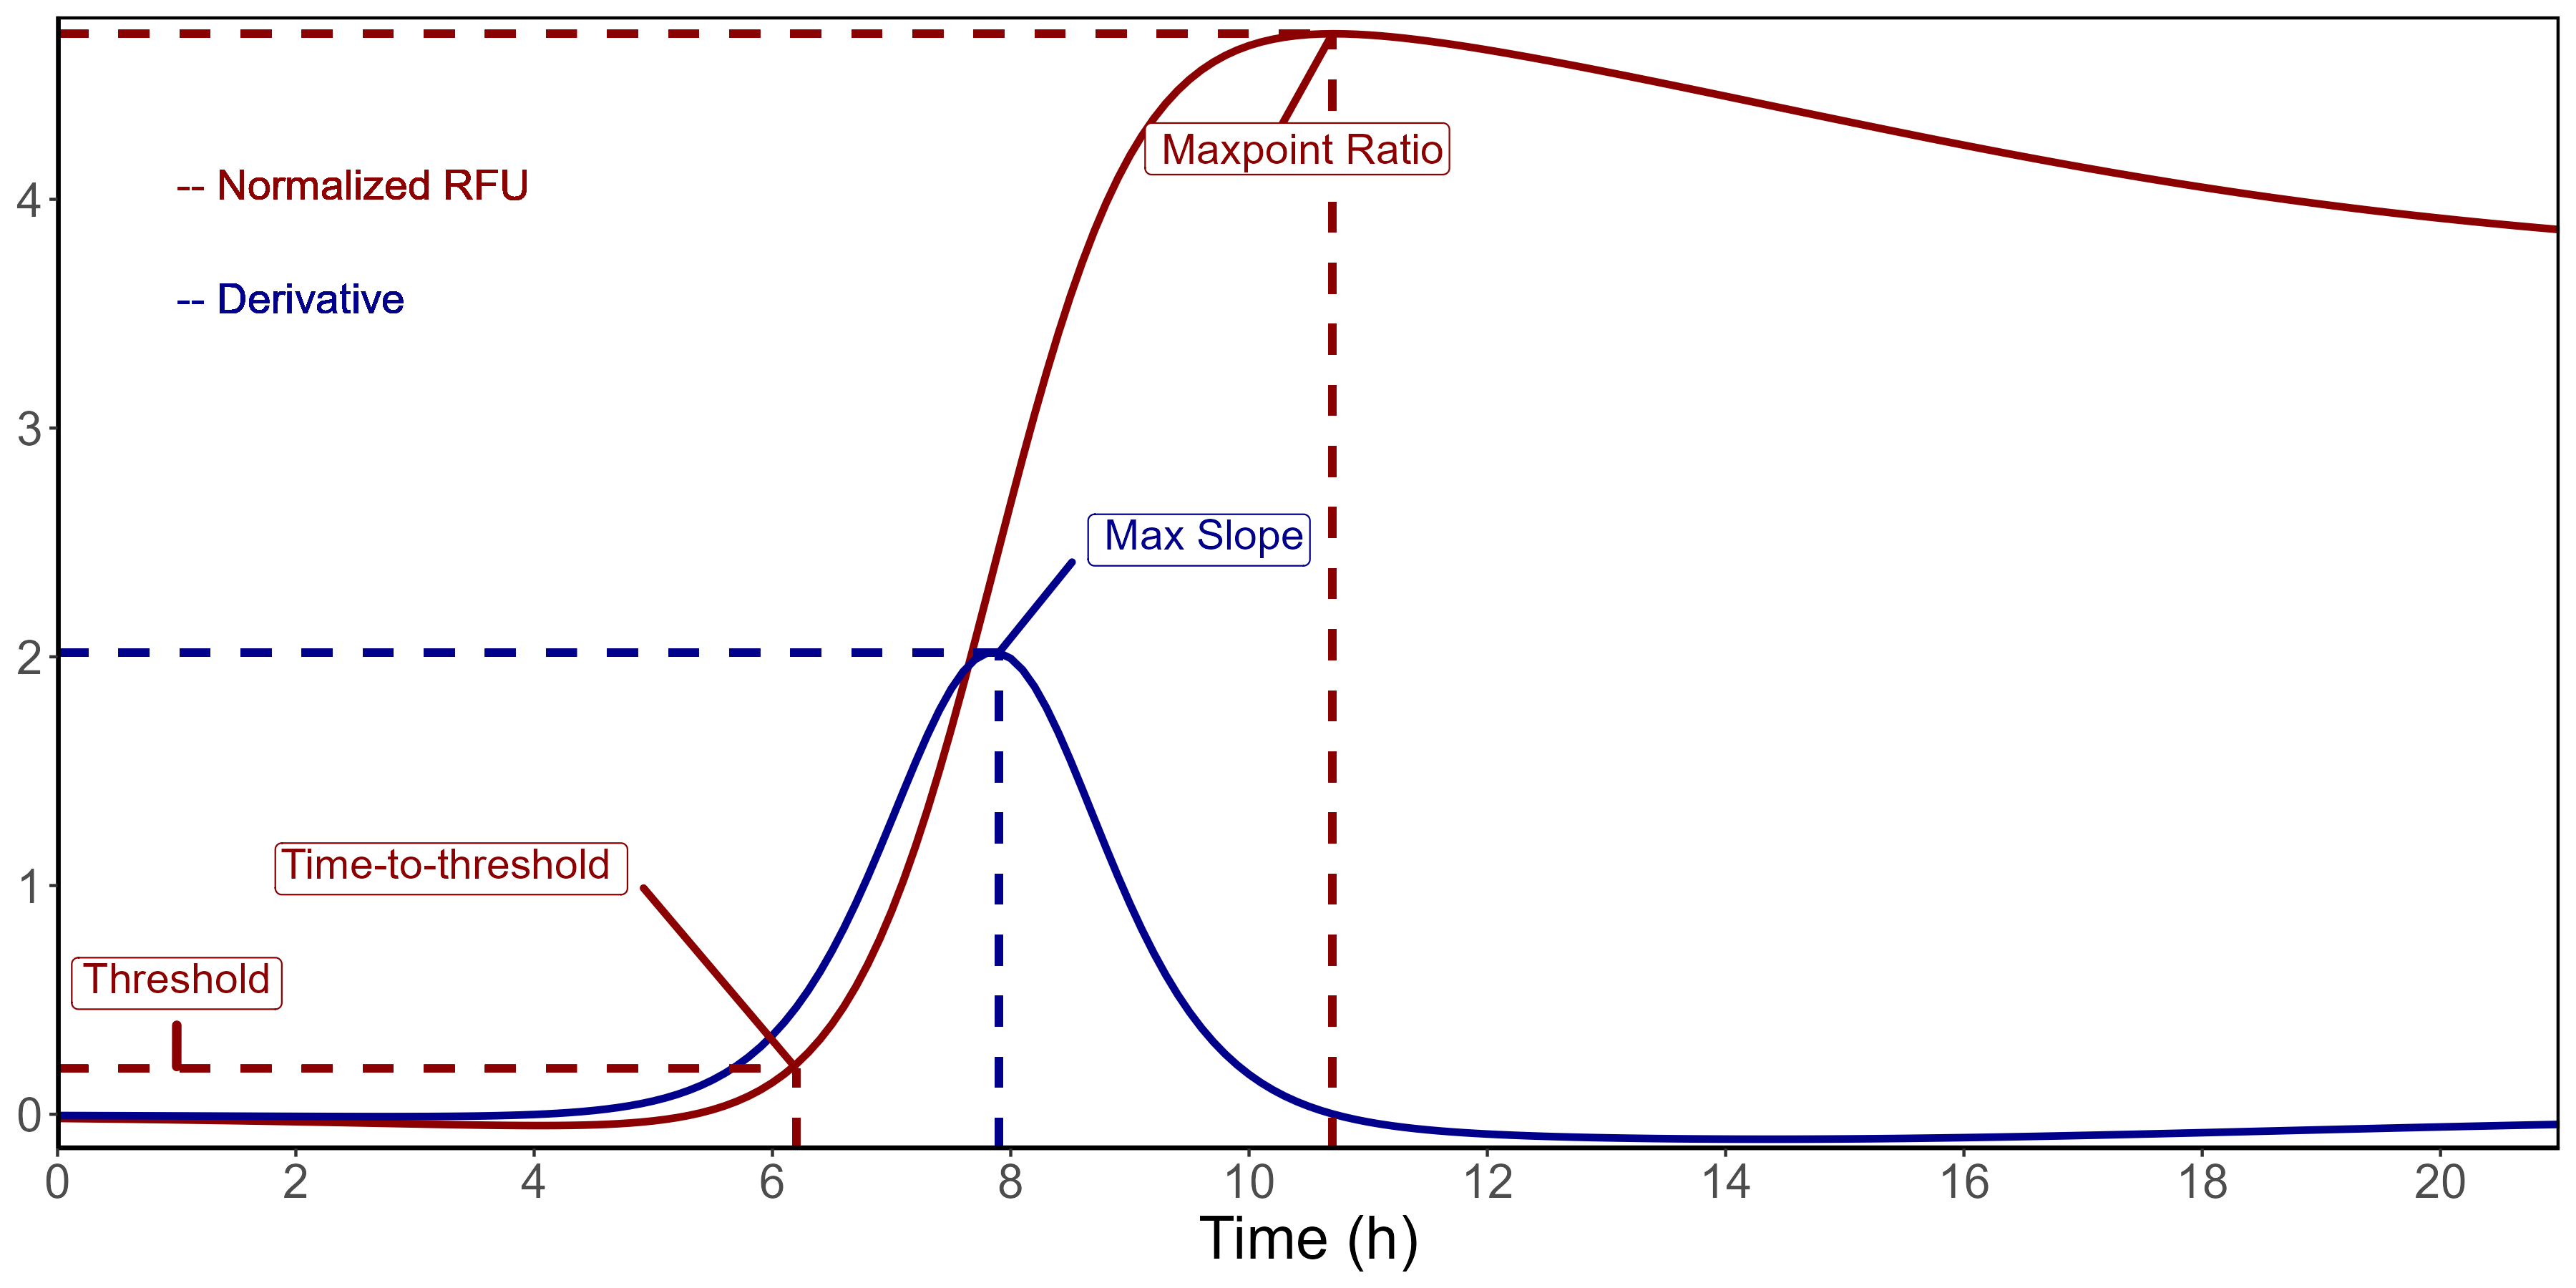
\includegraphics[width=\textwidth]{images/metric_example.png}
                \caption{Example graph highlighting the calculated metrics described above. The red curve represents a raw data curve that has been normalized against background. The maxpoint ratio is calculated as the maximum fluorescent value achieved in the normalized raw data. Time‐to‐threshold is determined as the time required to cross a given threshold (in this example, the threshold is set at 0.2). The blue curve represents the derivative of the raw data, and max slope is determined as the maximum of the derivative.}
                \label{fig:metrics}
            \end{figure}

        \subsubsection{Visualization}
            The ensuing goal of this package is visualizing RT-QuIC data. While there are many ways to represent this data, \textbf{quicR} includes two functions which provide a quick assessment of the reactions.
            \begin{enumerate}
                \item \textbf{plate\_view()}: accepts the output from the get\_real() function and get\_sample\_locations() function. Makes an 8$\times$12 or 16$\times$24 faceted plot depending on if the plate has 96 or 384 wells. Each facet shows the real-time data of each well.
                \item \textbf{plot\_metrics()}: requires the output of calculate\_metrics() and generates a boxplot of each sample's MPR, MS, RAF, and TtT.
            \end{enumerate}
        
    \section{Illustrative examples}
        To demonstrate the utility of \textbf{quicR}, we used a typical RT-QuIC run performed on a 96-well plate. The reaction was performed on a FLUOstar Omega plate reader (BMG Labtech, Ortenberg, Germany). The file was exported as an Excel workbook where the metadata appears on the first sheet and the raw data on the second.
        
        \subsection{Example Code}
            \# Step 1: Identify the raw file.\\
            file <- "example.xlsx"\\
            \# Step 2: Extract the raw data.\\
            raw <- get\_real(file)[[1]]\\
            \# Step 3: Normalize the data against the background.\\
            normal <- normalize\_RFU(raw, transposed = FALSE)\\
            \# Step 4: Extract the metadata.\\
            meta <- organize\_tables(file) |> convert\_tables()\\
            \# Step 5: Get sample locations.\\
            locations <- get\_sample\_locations(file)\\
            \# Step 6: Create the analyzed data frame.\\
            analyzed <- calculate\_metrics(normal, meta, dilution\_bool = TRUE)\\
            \# Step 7: Plot the analyzed data frame.\\
            plot\_metrics(analyzed)\\
            \# Step 8: Plot the plate view.\\
            plate\_view(raw, locations)\\

            Once the file name is identified, the function get\_real() is used to extract the raw data. This data is imported as a data frame with each sample designated as an individual column and the first column designated as time. Much of the downstream analysis works best with background-normalized data, so the raw data is then passed to the normalize\_RFU() function. This function accepts an integer as an argument for the desired cycle to be selected for background measurement. 
            
            Next, the metadata is extracted using the organize\_tables() and convert\_tables() functions. These take the metadata found on the first sheet of the Excel file and convert them into data frame columns. Finally, metrics are calculated and assigned to their given sample ID using calculate\_metrics(). This generates a data frame with sample IDs, dilution factors (if chosen), MPR's, MS's, RAF's, and TtT's.

            Once the proper variables have been defined, they can be used as input in the visualization functions. The analyzed data frame can be used as an argument in plot\_metrics() to generate a plot such as Figure \ref{fig:boxplot}. Additionally, the raw data and sample locations are used to plot the plate view as in Figure \ref{fig:plateview}.

            \begin{figure}[ht]
                \centering
                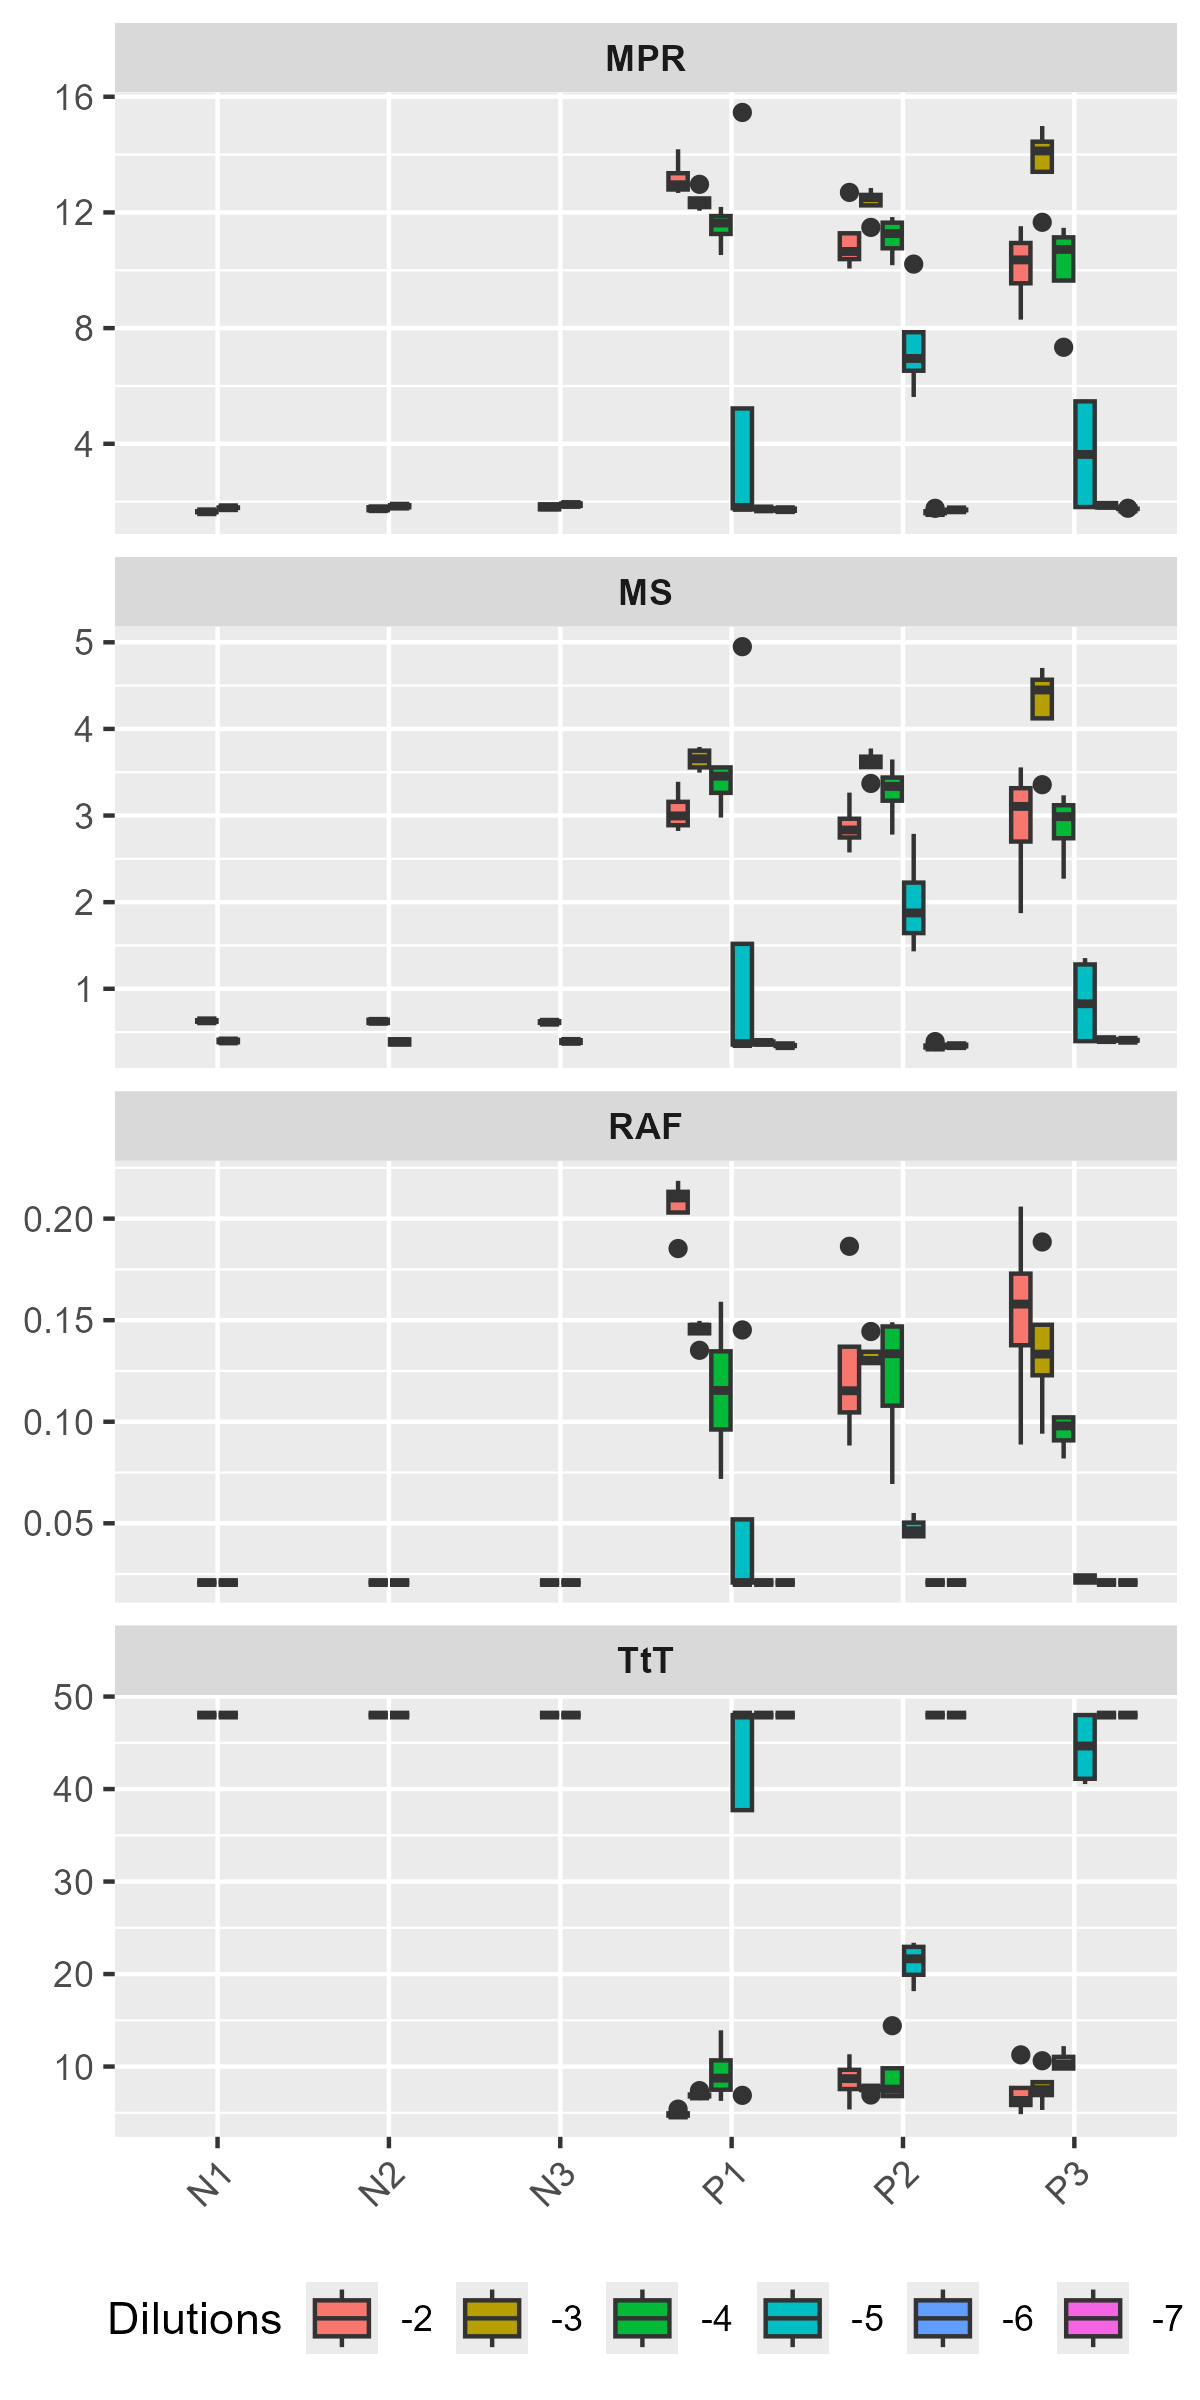
\includegraphics[width=\textwidth]{images/boxplot.png}
                \caption{Boxplot of the four critical metrics calculated by the \textbf{quicR} package.}
                \label{fig:boxplot}
            \end{figure}

            \begin{figure}[ht]
                \centering
                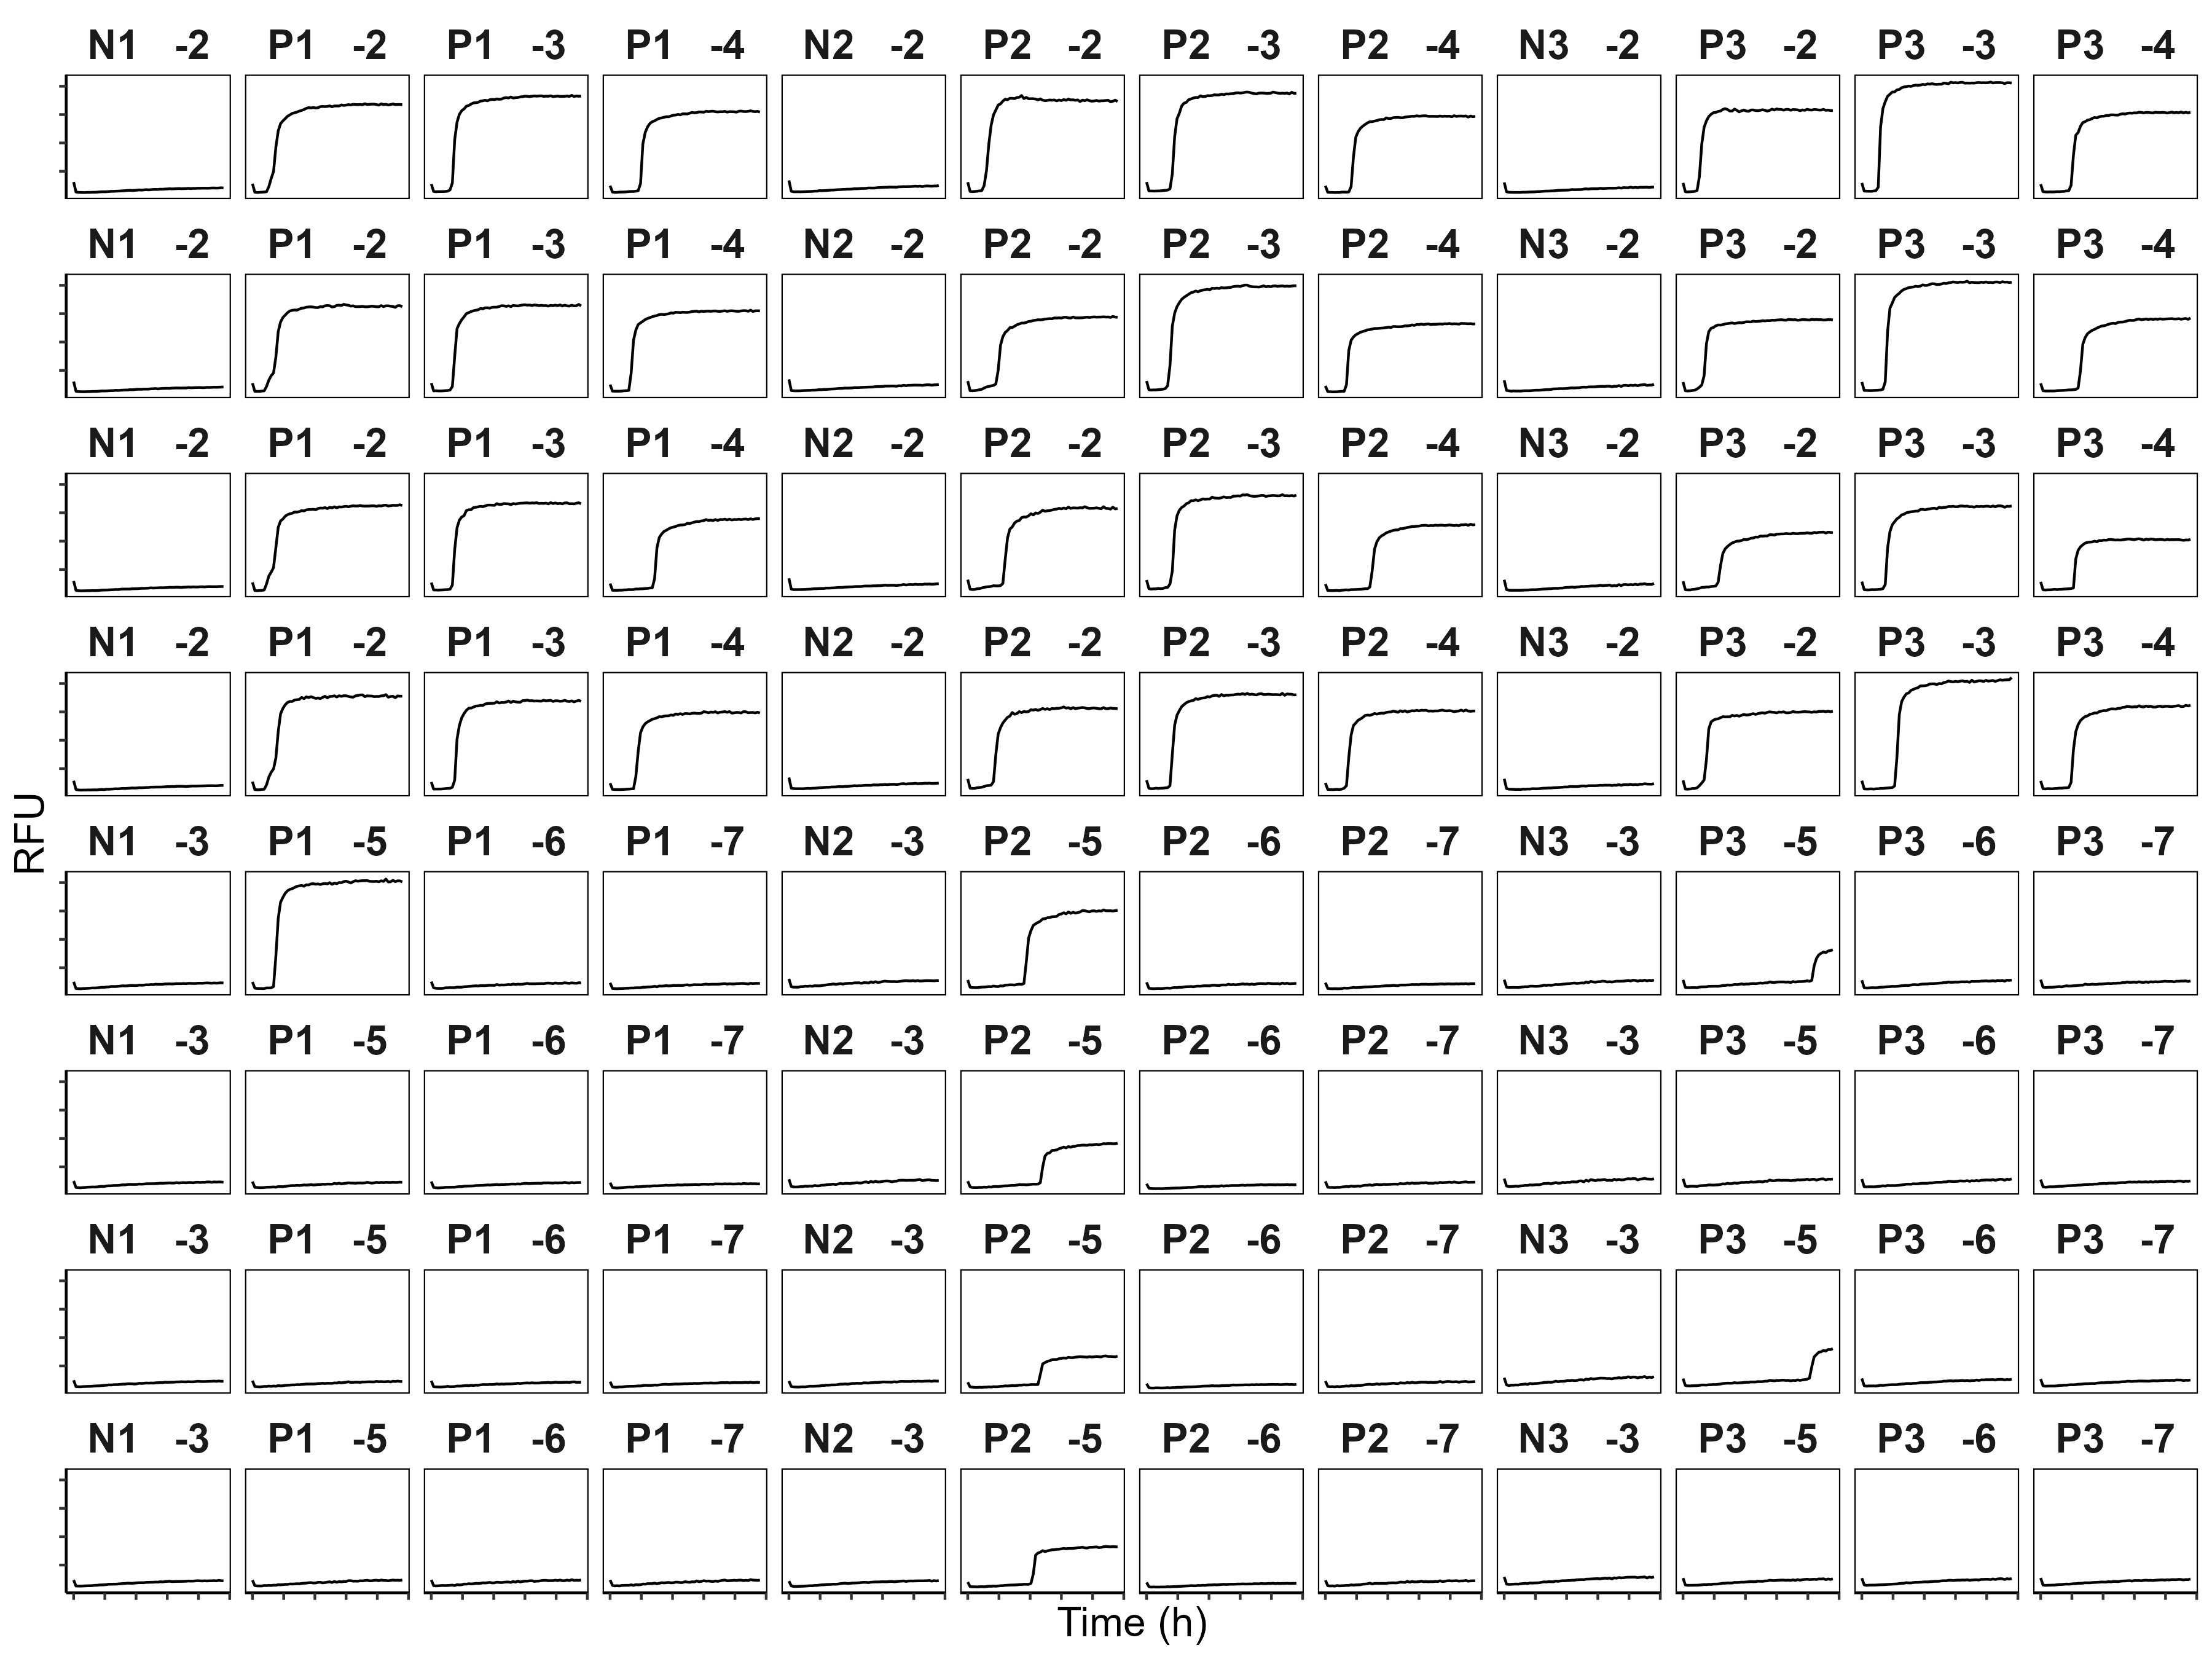
\includegraphics[width=\textwidth]{images/plate_view.png}
                \caption{Plate view of RT-QuIC. Wells are identified with a sample ID and dilution factor separated by an optional delimiter (in this case, a whitespace).}
                \label{fig:plateview}
            \end{figure}
            
    \section{Impact}
        The \textbf{quicR} package represents a significant advancement in the standardization and reproducibility of RT-QuIC data analysis. By integrating key metrics such as time-to-threshold (TtT) \cite{Orru2015}, maxpoint ratio (MPR) \cite{Rowden2023}, and maximum slope (MS) \cite{Henderson2015}, \textbf{quicR} addresses critical gaps in the field, providing researchers and diagnosticians with a robust toolkit for interpreting RT-QuIC data.

        One of the primary strengths of \textbf{quicR} lies in its streamlined workflow and user-centric design. The package leverages R’s powerful ecosystem and the tidyverse to create high-quality, customizable visualizations, ensuring accessibility for a wide range of users, from experienced data scientists to wet-lab researchers unfamiliar with programming. Additionally, the incorporation of open-source principles allows the broader scientific community to contribute to its development, fostering innovation and adaptability.

        Despite these strengths, there are limitations to consider. Currently, \textbf{quicR} is tailored to data exported from the MARS software, which may limit its applicability to researchers using alternative microplate readers. Future iterations of the package could expand compatibility by incorporating functions to handle diverse data formats. Furthermore, while \textbf{quicR} includes robust visualization tools, users seeking highly specialized plots like those made by Li, et al.\cite{Li2025} may require additional customization beyond the package’s default capabilities.

        Another avenue for improvement lies in the standardization of RT-QuIC diagnostic criteria. \textbf{quicR} provides tools to calculate key metrics, but consensus on thresholds and interpretations remains a challenge for the field \cite{Rowden2023}. Collaborative efforts among researchers and clinicians are necessary to define universal criteria, enabling \textbf{quicR} to fully realize its potential as a diagnostic aid. Diagnostic determinations could easily be built into the library, but a larger consensus within the research community will need to be reached to warrant inclusion.

    \section{Conclusions}
        \textbf{quicR} offers a powerful solution for the cleaning, analysis, and visualization of RT-QuIC data, addressing critical needs in a rapidly evolving field. By enabling consistent data handling and interpretation, \textbf{quicR} lays the groundwork for improved diagnostic consistency and reproducibility. The package's open-source nature ensures that it will continue to evolve, integrating new insights and technologies as they emerge.

        As RT-QuIC technology advances, tools like \textbf{quicR} will play a pivotal role in bridging the gap between assay development and practical application. By equipping researchers with reliable, standardized tools, \textbf{quicR} not only supports the study of prion and protein misfolding disorders but also serves as a model for the development of software solutions in other diagnostic fields.

    \section*{Acknowledgements}
        Special thanks to Beni Altmann at The Comprehensive R Archive Network (CRAN) for help during the submission process to CRAN. We thank Tiffany Wolf and Marc Schwabenlander for their support through the Minnesota Center for Prion Research and Outreach. We would like to acknowledge Suzanne Stone and Sarah Gresch for maintaining lab operations.

    %% The Appendices part is started with the command \appendix;
    %% appendix sections are then done as normal sections
    %% \appendix

    \bibliographystyle{elsarticle-num} 
    \bibliography{references}

\end{document}
\endinput
